         \chapter{Meganiese energie}\fancyfoot[LO,RE]{Fisika: Mechanics} \label{chap:energy}
    \setcounter{figure}{1}
    \setcounter{subfigure}{1}
    \label{1fc5ba69690764517c30802fdf7b1905}
         \section{Inleiding}
    \nopagebreak
            \label{m38784} $ \hspace{-5pt}\begin{array}{cccccccccccc}   
\includegraphics[width=0.75cm]{col11305.imgs/summary_fullmarks.png} &   \end{array} $ \hspace{2 pt}\raisebox{-5 pt}{} {(section shortcode: P10104 )} \par 
            \label{m38784*id7521}
Alle voorwerpe het energie. Die woord energie is afgelei van die Griekse woord energeia ($έ\nu έ\rho \gamma \epsilon \iota \alpha $) wat aktiwiteit of handeling beteken. Energie en massa gaan hand aan hand en kan nie geskep of vernietig word nie. In hierdie hoofstuk gaan ons kyk na gravitasie potensiële energie en kinetiese energie. \label{m38784*cid4}
            \section{Potensi\"{e}le energie}
            \nopagebreak
Die potensi\"{e}le energie van ‘n voorwerp word oor die algemeen gedefinieer as die energie wat ‘n voorwerp het as gevolg van sy posisie relatief tot ander voorwerpe waarmee dit in wisselwerking is. Daar is verskillende soorte potensiële energie soos gravitasie potensi\"{e}le energie, elektriese potensile energie en chemiese potensiële energie om maar net ‘n paar te noem. Hierdie afdeling ondersoek gravitasie potensi\"{e}le energie. 
\Definition{ Potensi\"{e}le energie } { Potensi\"{e}le energie is die energie wat ‘n voorwerp het as gevolg van sy posisie of toestand.} 

\Definition{Gravitasie Potensi\"{e}le energie, $E_{P}$ }{ Gravitasie potensi\"{e}le energie is die energie wat ‘n voorwerp het as gevolg van sy posisie in ‘n gravitasieveld relatief tot ‘n sekere verwysingspunt. \\
 Simbool: $E_{P}$ \hspace{2cm} S.I. Eenheid: $\text{J}$}

      \label{m38784*id66167}Waar die aarde ter sprake is, is \textsl{gravitasie} potensi\"{e}le energie die energie wat ‘n voorwerp het as gevolg van sy posisie bo die aarde se oppervlak. Die simbool ${E}_{P}$ verwys na gravitasie potensiële energie. Dit gebeur gereeld dat die woorde potensiële energie gebruik word wanneer die bedoeling eerder \textsl{gravitasie} potensiële energie is. Gravitasie potensi\"{e}le energie word as volg gedefinieer:\\
      \label{m38784*uid45}\nopagebreak\noindent{}
    \begin{equation}
    {E}_{P}=mgh
      \end{equation}
      \label{m38784*id66223}waar
${E}_{P}$ = potensi\"{e}le energie (in joules, J, gemeet)\par 
      \label{m38784*id66229}m = massa van die voorwerp (in kg gemeet)\par 
      \label{m38784*id66234}g = gravitasieversnelling ($9,8\phantom{\rule{2pt}{0ex}}\text{m}\ensuremath{\cdot}\text{s}{}^{-2}$)\par 
      \label{m38784*id66266}h = vertikale hoogte van die verwysingspunt (gemeet in m)\par 
      \label{m38784*eip-306}
\Tip{Jy sal agterkom dat potensiële energie partykeer as PE uitgedruk word. Ons gaan dit nie in hierdie boek so gebruik nie, maar jy sal dit dalk in ander boeke sien. }

Jy kan gravitasieversnelling, g, as ‘n konstante beskou. Jy sal meer daaroor leer in grade 11 en 12. 


Kom ons kyk na die geval van ‘n tas, met ‘n massa van $1\phantom{\rule{2pt}{0ex}}\text{kg}$, wat bo-op ‘n $2\phantom{\rule{2pt}{0ex}}\text{m}$ ho\"{e} kas geb\^{e}re word. Deur die tas teen die gravitasiekrag op te tel, gee ons vir die tas potensi\"{e}le energie. Ons kan die gravitasie potensi\"{e}le energie uitwerk deur die vergelyking wat hier bo gedefinieer is te gebruik:
\begin{eqnarray*}
E_{P} & = & mgh \\
& = & (1)(9,8)(2) = 19,6 \text{ J}
\end{eqnarray*}
As die tas van die kas sou afval, verloor dit sy potensiële energie. Halfpad op pad vloer toe, sou die tas die helfte van sy potensiële energie verloor het en sal daar net $9,8\phantom{\rule{2pt}{0ex}}\text{J}$ oorbly. 
\begin{eqnarray*}
E_{P} & = & mgh \\
& = & (1)(9,8)(1) = 9,8 \text{ J} \\
\end{eqnarray*}
Wanneer die tas op die grond val, sal dit al sy potensi\"{e}le energie verloor het en die potensi\"{e}le energie sal nul wees.
\begin{eqnarray*}
E_{P} & = & mgh \\
& = & (1)(9,8)(0) = 0 \text{ J} \\
\end{eqnarray*}

Die voorbeeld wys vir ons dat ‘n voorwerp sy maksimum potensi\"{e}le energie by ‘n maksimum hoogte bereik en potensi\"{e}le energie verloor as dit val.

      \label{m38784*id66298}
    \setcounter{subfigure}{0}
\begin{figure}[H]
\begin{center}
\begin{pspicture}(0,0)(3,5)
%\psgrid[subgriddiv=1,griddots=10,gridlabels=7pt]
\psframe[linewidth=2pt](0,0)(2,4)
%suitcase on top
\psframe[linewidth=1.5pt](1.2,4)(2,4.5)
\pscurve[linewidth=2pt](1.4,4.5)(1.6,4.7)(1.8,4.5)
%suitcase at bottom
\psframe[linewidth=1.5pt](2.2,0)(3,0.5)
\pscurve[linewidth=2pt](2.4,0.5)(2.6,0.7)(2.8,0.5)
\psline[linestyle=dashed](2,4)(3,4)
\psline[linestyle=dotted]{->}(2.6,4)(2.6,0.8)
\rput[l](3.1,3.8){$E_{P}$ = mgh = (1)(9,8)(2) = 19,6 J}
\rput[l](3.1,-0.2){$E_{P}$ = mgh = (1)(9,8)(0) = 0 J}
\rput[l](3.1,4.2){Vlak van maksimum potensi\"{e}le energie}
\rput[l](3.1,0.3){Vlak van minimum potensi\"{e}le energie}
\end{pspicture}
\end{center}
\end{figure}      
      \par 
\label{m38784*secfhsst!!!underscore!!!id939}\vspace{.5cm} 



      \noindent
\begin{wex}{Gravitasie potensi\"{e}le energie}{‘n Baksteen met ‘n massa van 1kg word tot bo-op ‘n 4m ho\"{e} dak gehys. Dit val van die dak af terug grond toe. Bereken die gravitasie potensi\"{e}le energie van die baksteen bo-op die dak en op die grond nadat dit geval het.}
{
\westep{Ontleed die vraag en bepaal watter inligting vir jou gegee is.}
\begin{itemize}
\item{Die massa van die baksteen is $m$ = 1~kg}
\item{Die hoogte wat dit opgehys is, is $h$ = 4~m}
\end{itemize}
Alle eenhede is in SI eenhede

\westep{Ontleed die vraag en bepaal wat gevra word}
\begin{itemize}
\item Ons word gevra om die potensi\"{e}le energie van die baksteen te bereken terwyl dit na die dak gehys word.
\item Ons moet ook die potensi\"{e}le energie van die baksteen bereken sodra dit weer op die grond is.
\end{itemize}

\westep{Identify the type of potential energy involved}
Since the brick is being lifted we are dealing with gravitational potential energy. To work out $E_{P}$, we need to know the mass of the object and the height lifted. As both of these are given, we just substitute them into the equation for $E_{P}$.

\westep{Substitute and calculate}
\begin{eqnarray*}
E_{P} & = & mgh \\
&=& (1)(9,8)(4) \\
&=& 39,2 \text{ J}
\end{eqnarray*}}
\end{wex}

    %\noindent
\begin{exercises}{Gravitational Potential Energy }
            \nopagebreak
      \label{m38784*id66588}\begin{enumerate}[noitemsep, label=\textbf{\arabic*}. ] 
            \label{m38784*uid50}\item Beskryf die ooreenkoms tussen ‘n voorwerp se gravitasie potensi\"{e}le energie en sy:
\label{m38784*id66604}\begin{enumerate}[noitemsep, label=\textbf{\alph*}. ] 
            \label{m38784*uid51}\item massa en 
\label{m38784*uid52}\item hoogte bo ‘n verwysingspunt.
\end{enumerate}
                \label{m38784*uid53}\item ‘n Seun met ‘n massa van $30\phantom{\rule{2pt}{0ex}}\text{kg}$, klim op die motorhuis se dak. Die dak is $2,5\phantom{\rule{2pt}{0ex}}\text{m}$ van die grond af. He now jumps off the roof and lands on the ground.
\label{m38784*id66646}\begin{enumerate}[noitemsep, label=\textbf{\alph*}. ] 
            \label{m38784*uid54}\item Hoeveel potensi\"{e}le energie het die seun bygekry deur op die dak te klim?
\label{m38784*uid55}\item Die seun spring nou van die dak af. Wat is die potensi\"{e}le energie van die seun wanneer hy $1 \text{m}$ van die grond af is?
\label{m38784*uid56}\item Wat is die potensi\"{e}le energie van die seun op die grond?
\end{enumerate}
                \label{m38784*uid57}\item ‘n Stapper, met ‘n massa van $70 \text{ kg}$ klim ‘n berg wat $800\phantom{\rule{2pt}{0ex}}\text{m}$ bo seespie\"{e}l is, om in die eerste oornaghut bo-op die berg te gaan slaap. Op dag twee stap sy na die tweede oornaghut wat $500\phantom{\rule{2pt}{0ex}}\text{m}$ bo seespie\"{e}l is. Op dag drie keer sy terug na haar beginpunt $200\phantom{\rule{2pt}{0ex}}\text{m}$ bo seespie\"{e}l.
\label{m38784*id66702}\begin{enumerate}[noitemsep, label=\textbf{\alph*}. ] 
            \label{m38784*uid58}\item Wat is die potensi\"{e}le energie van die stapper by die eerste oornaghut (relatief tot seespie\"{e}l)?
\label{m38784*uid59}\item Hoeveel potensi\"{e}le energie het die stapper verloor gedurende die tweede dag?
\label{m38784*uid60}\item Hoeveel potensi\"{e}le energie het die stapper aan die begin van haar staptog gehad (relatief tot seespie\"{e}l)?
\label{m38784*uid61}\item Hoeveel potensi\"{e}le energie het die stapper aan die einde van die staptog gehad toe sy weer by haar oorspronklike beginpunt aangekom het?
\end{enumerate}
                \end{enumerate}
  \label{m38784**end}
\par \raisebox{-0.2em}{
\includegraphics[height=1em]{../icons/www.pdf}} Find the answers with the shortcodes:
 \par \begin{tabular}[h]{cccccc}
 (1.) lxE  &  (2.) lxm  &  (3.) lxy  & \end{tabular}
\end{exercises}


         \section{Kinetiese energie}
    \nopagebreak
            \label{m38785} $ \hspace{-5pt}\begin{array}{cccccccccccc}   
\includegraphics[width=0.75cm]{col11305.imgs/summary_fullmarks.png} &   \end{array} $ \hspace{2 pt}\raisebox{-5 pt}{} {(section shortcode: P10105 )} \par 
\Definition{ Kinetiese Energie, $E_{K}$ } {Kinetiese energie is die energie wat ‘n voorwerp het as gevolg van sy beweging.\\
Simbool: $E_{K}$ S.I. Eenheid: J} 
      \end{tabular*}
      \end{definition}
      \label{m38785*id66796}Kinetiese energie is die energie wat ‘n voorwerp het as gevolg van sy beweging. Dit beteken dat enige bewegende voorwerp kinetiese energie het. Kinetiese energie word as volg gedefinieer:
    \begin{equation}
    {E}_{K}=\frac{1}{2}m{v}^{2}
      \end{equation}

waar $E_{K}$ die kinetiese energie is (gemeet in joules J) \\

m = massa van die voorwerp (gemeet in kg) \\

v = snelheid van die voorwerp (gemeet in $\text{m} \cdot \text{s}^{-1}}$). \\

Die kinetiese energie $E_{K}$ van ‘n voorwerp hang daarom af van sy massa en snelheid. Hoe vinniger ‘n voorwerp beweeg, en hoe groter die massa is, hoe meer kinetiese energie het dit. ‘n Vragmotor van $2 000\phantom{\rule{2pt}{0ex}}\text{kg}$, wat teen $100\phantom{\rule{2pt}{0ex}}\text{km}\ensuremath{\cdot}\text{hr}{}^{-1}$ beweeg sal dus meer kinetiese energie h\^{e} as ‘n motor van $500\phantom{\rule{2pt}{0ex}}\text{kg}$, wat ook teen $100\phantom{\rule{2pt}{0ex}}\text{km}\ensuremath{\cdot}\text{hr}{}^{-1}$ beweeg. 
      \label{m38785*eip-368}
\Tip{Partykeer word die simbool $\text{KE}$. gebruik vir kinetiese energie. Dit is ‘n ander manier om kinetiese energie uit te druk. Ons gaan dit nie in hierdie handboek gebruik nie, maar jy mag dit dalk in ander boeke sien.}
      \label{m38785*uid62}\nopagebreak\noindent{}

      \label{m38785*id66902}Dink weer aan die $1\phantom{\rule{2pt}{0ex}}\text{kg}$ tas op die hangkas wat ons vroe\"{e}r bespreek het. Wanneer die tas bo-op die kas lê, sal dit geen kinetiese energie hê nie, omdat dit nie beweeg nie.
\begin{eqnarray*}
E_{K} &=& \frac{1}{2}mv^{2} \\
& = & \frac{1}{2}(1)(0)^{2} = 0 \text{ J}.
\end{eqnarray*}
Wanneer die tas val kry dit snelheid (dit val vinniger) totdat dit die grond bereik teen ‘n maksimum snelheid. Soos die snelheid vermeerder, vermeerder die kinetiese energie. Die kinetiese energie van die tas sal aanhou verhoog tot dit op sy maksimum kom wanneer die tas die grond tref. As die tas ‘n snelheid van 6,26 $\text{m}  \cdot \text{s}^{-1}}$ het wanneer dit die grond tref, is sy kinetiese energie:
\begin{eqnarray*}
E_{K} &=& \frac{1}{2}mv^{2} \\
& = & \frac{1}{2}(1)(6,26)^{2} = 19,6 \text{ J}.
\end{eqnarray*}

      \label{m38785*id66909}
    \setcounter{subfigure}{0}
	\begin{figure}[H] % horizontal\label{m38785*id66912}
\begin{center}
\begin{pspicture}(0,0)(3,5)
%\psgrid[subgriddiv=1,griddots=10,gridlabels=7pt]
\psframe[linewidth=2pt](0,0)(2,4)
%suitcase on top
\psframe[linewidth=1.5pt](1.2,4)(2,4.5)
\pscurve[linewidth=2pt](1.4,4.5)(1.6,4.7)(1.8,4.5)
%suitcase at bottom
\psframe[linewidth=1.5pt](2.2,0)(3,0.5)
\pscurve[linewidth=2pt](2.4,0.5)(2.6,0.7)(2.8,0.5)
\psline[linestyle=dashed](2,4)(3,4)
\psline[linestyle=dotted]{->}(2.6,4)(2.6,0.8)
\rput[l](3.1,3.8){$E_{K}~=~\frac{1}{2}mv^2~=(\frac{1}{2})(1)(0)^2 = ~0 \text{ J}$}
\rput[l](3.1,-0.2){$E_{K}~=~\frac{1}{2}mv^2~=(\frac{1}{2})(1)(6,26)^2 = ~19,6 \text{ J}$}
\rput[l](3.1,4.2){Vlak van minimum kinetiese energie}
\rput[l](3.1,0.3){Vlak van maksimum kinetiese energie}
\end{pspicture}
\end{center}
 \end{figure}       
      \par 
\label{m38785*secfhsst!!!underscore!!!id1079}\vspace{.5cm} 
      \noindent
\begin{wex}{Bereken Kinetiese Energie}{‘n 1kg baksteen val van ‘n 4m hoë dak af. Dit tref die grond teen ‘n snelheid van \ms. Wat is die kinetiese energie van die baksteen toe dit begin val het en toe dit die grond getref het.}
{\westep{Ontleed die vraag en bepaal watter inligting vir jou gegee is.}
\begin{itemize}
\item Die massa van die baksteen is $m$ = 1 kg
\item Die snelheid van die baksteen op die grond is $v_{bottom}$ = 8,85 \ms
\end{itemize}
Beide hierdie waardes is in die korrekte eenhede so ons hoef hulle nie om te skakel nie.

\westep{Ontleed die vraag en bepaal wat gevra word.}
Ons moet uitvind wat die kinetiese energie van die baksteen op die dak en op die grond is. Die definisie s\^{e} dat om $E_{k}$ uit te werk ons die massa en die snelheid van die voorwerp moet h\^{e} en albei hierdie waardes is vir ons gegee.

\westep{Bereken die kinetiese energie by die hoogste punt}
Aangesien die baksteen nie beweeg op die dak nie, is die kinetiese energie nul.
\westep{Vervang waardes en bereken kinetiese energie}
\begin{eqnarray*}
E_{K} & = & \frac{1}{2}mv^2 \\
&=& \frac{1}{2}(1\ \ekg)(8,85\ \ems)^2 \\
&=& 39,2 \text{ J}
\end{eqnarray*}}
\end{wex}
    \noindent
      \label{m38785*uid65}
            \subsection*{Kontroleer eenhede}
            \nopagebreak
        \label{m38785*id67277}Volgens die vergelyking vir kinetiese energie behoort die eenheid $\text{kg}\ensuremath{\cdot}\text{m}{}^{2}\ensuremath{\cdot}\text{s}{}^{-2}$. te wees. Ons kan bewys dat hierdie eenheid gelyk is aan joule – die eenheid vir energie. 
        \label{m38785*id67329}\nopagebreak\noindent{}
    \begin{equation}
    \begin{array}{cccc}\hfill \left(\text{kg}\right){\left(\text{m}\ensuremath{\cdot}{\text{s}}^{-1}\right)}^{2}& =& \left(\text{kg}\ensuremath{\cdot}\text{m}\ensuremath{\cdot}{\text{s}}^{-2}\right)\ensuremath{\cdot}\text{m}\hfill & \\ & =& \phantom{\rule{0.166667em}{0ex}}\text{N}\ensuremath{\cdot}\phantom{\rule{0.166667em}{0ex}}\text{m}\hfill & \left(\text{want\; krag}\phantom{\rule{2pt}{0ex}}\left(\text{N}\right)=\text{massa}\phantom{\rule{2pt}{0ex}}\left(\text{kg}\right)\ensuremath{\times}\text{acceleration}\phantom{\rule{2pt}{0ex}}\left(\text{m}\ensuremath{\cdot}{\text{s}}^{-2}\right)\right)\hfill \\ & =& \phantom{\rule{0.166667em}{0ex}}\text{J}\hfill & \left(\text{Werk}\phantom{\rule{2pt}{0ex}}\left(\text{J}\right)=\text{Krag}\phantom{\rule{2pt}{0ex}}\left(\text{N}\right)\ensuremath{\times}\text{distance}\phantom{\rule{2pt}{0ex}}\left(\text{m}\right)\right)\hfill \end{array}
      \end{equation}
        \label{m38785*id67613}Ons kan dieselfde doen om te bewys dat die eenheid vir potensi\"{e}le energie gelyk is aan joule:\par 
        \label{m38785*id67619}\nopagebreak\noindent{}
          
    \begin{equation}
    \begin{array}{ccc}\hfill \left(\text{kg}\right)\left(\text{m}\ensuremath{\cdot}{\text{s}}^{-2}\right)\left(\text{m}\right)& =& \phantom{\rule{0.166667em}{0ex}}\text{N}\ensuremath{\cdot}\phantom{\rule{0.166667em}{0ex}}\text{m}\hfill \\ & =& \phantom{\rule{0.166667em}{0ex}}\text{J}\hfill \end{array}
      \end{equation}
\par
            \label{m38785*secfhsst!!!underscore!!!id1394}\vspace{.5cm} 

      \noindent
\begin{wex}{Kombineer eenhede en energie berekeninge }{‘n Koe\"{e}l met ‘n massa van 150g word geskiet met ‘n trompsnelheid van 960~\ms. Bereken die kinetiese energie van die koe\"{e}l.}
{\westep{Ontleed die vraag en bepaal watter inligting vir jou gegee is.}
\begin{itemize}
\item Die massa van die koe\"{e}l word vir ons gegee as $m$ = 150~g. Dit is nie die eenheid waarin ons die massa wil h\^{e} nie. Ons moet dit omskakel na kg.
\begin{eqnarray*}
\text{Massa in grams} \div 1000 &=& \text{Massa in kg}\\
150~\text{g} \div 1000 &=& 0,150~\text{kg}
\end{eqnarray*}

\item Die aanvangsnelheid waarmee die koe\"{e}l uit die loop geskiet word, die trompsnelheid, word vir ons gegee as $v$ = 960~\ms.
\end{itemize}
\westep{Ontleed die vraag en bepaal wat gevra word.}
\begin{itemize}
\item Ons moet uitvind wat die kinetiese energie is.
\end{itemize}

\westep{Vervang waardes en bereken.}
We just substitute the mass and velocity (which are known) into the equation for kinetic energy:
\begin{eqnarray*}
E_{K} & = & \frac{1}{2}mv^2 \\
&= & \frac{1}{2}(0,150)(960)^2 \\
&=& 69\,120 \text{ J}
\end{eqnarray*}}
\end{wex}
    \noindent
\label{m38785*secfhsst!!!underscore!!!id1491}
\begin{exercises}{Kinetiese Energie }
            \nopagebreak
        \label{m38785*id68123}\begin{enumerate}[noitemsep, label=\textbf{\arabic*}. ] 
            \label{m38785*uid69}\item Beskryf die ooreenkoms tussen ‘n voorwerp se kinetiese energie en sy:
\label{m38785*id68139}\begin{enumerate}[noitemsep, label=\textbf{\alph*}. ] 
            \label{m38785*uid70}\item  massa en
\label{m38785*uid71}\item snelheid
\end{enumerate}
                \label{m38785*uid72}\item ‘n Klip met ‘n massa van $100 \text{g}$ word in die lug opgegooi. Dit het ‘n aanvangsnelheid van $3\phantom{\rule{2pt}{0ex}}\text{m}\ensuremath{\cdot}\text{s}{}^{-1}$. Bereken die kinetiese energie:
\label{m38785*id68206}\begin{enumerate}[noitemsep, label=\textbf{\alph*}. ] 
            \label{m38785*uid73}\item wanneer dit die persoon se hand verlaat.
\label{m38785*uid74}\item  wanneer dit sy draaipunt bereik.
\end{enumerate}
                \label{m38785*uid75}\item ‘n Motor met ‘n massa van $700\phantom{\rule{2pt}{0ex}}\text{kg}$ beweeg teen ‘n konstante snelheid van $100\phantom{\rule{2pt}{0ex}}\text{km}\ensuremath{\cdot}\text{hr}{}^{-1}$. Bereken die kinetiese energie van die motor.
\end{enumerate}
  \label{m38785**end}
\par \raisebox{-0.2em}{
\includegraphics[height=1em]{../icons/www.pdf}} Find the answers with the shortcodes:
 \par \begin{tabular}[h]{cccccc}
 (1.) lad  &  (2.) law  &  (3.) lav  & \end{tabular}
\end{exercises}
         \section{Meganiese energie}
    \nopagebreak
            \label{m38786} $ \hspace{-5pt}\begin{array}{cccccccccccc}   
\includegraphics[width=0.75cm]{col11305.imgs/summary_fullmarks.png} &   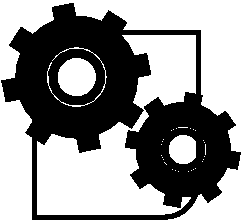
\includegraphics[width=0.75cm]{col11305.imgs/summary_simulation.png} &   \end{array} $ \hspace{2 pt}\raisebox{-5 pt}{} {(section shortcode: P10106 )} \par 
      \label{m38786*id68299}Meganiese energie, ${E}_{M}$, is eenvoudig die som van die gravitasie potensi\"{e}le energie (${E}_{P}$) en die kinetiese energie (${E}_{K}$). Meganiese energie word gedefinieer as:
      \label{m38786*uid76}\nopagebreak\noindent{}
    \begin{equation}
    {E}_{M}={E}_{P}+{E}_{K}
      \end{equation}
      \label{m38786*uid77}\nopagebreak\noindent{}
    \begin{equation}
    \begin{array}{ccc}\hfill {E}_{M}& =& {E}_{P}+{E}_{K}\hfill \\ \hfill {E}_{M}& =& mgh+\frac{1}{2}m{v}^{2}\hfill \end{array}
      \end{equation}
      \label{m38786*eip-384}
\Tip{You may see mechanical energy written as $U$. We will not use this notation in this book, but you should be aware that this notation is sometimes used.}
      \label{m38786*uid78}
            

\section{Behoud van meganiese energie }
            \nopagebreak
\Definition{ Behoud van Energie } { Die Beginsels van of die Wet van Behoud van Energie: Energie kan nie geskep of vernietig word nie, dit kan slegs van een vorm na ‘n ander verander word.  } 
        \label{m38786*id68483}Tot dusver het ons na twee soorte energie gekyk: gravitasie potensiële energie en kinetiese energie. Die som van die gravitasie potensiële energie en kinetiese energie word meganiese energie genoem. In ‘n geslote sisteem waar daar geen eksterne kragte uitwerking op ‘n voorwerp het nie, sal die meganiese energie konstant bly. Met ander woorde dit sal nie verander nie (sal nie meer of minder word nie). Dit word die Wet van Behoud van Meganiese Energie genoem. 

\Definition{ Behoud van meganiese energie } { Die Wet van Behoud van Meganiese Energie:  Die totale hoeveelheid meganiese energie in ‘n geslote sisteem vry van die uitwerking van eksterne kragte (bv. wrywing, lugweerstand), bly konstant.  } 

Dit beteken dat potensiële energie kinetiese energie kan word, of andersom, maar energie kan nie net verdwyn nie. Byvoorbeeld: Wanneer daar geen lugweerstand is nie, sal die meganiese energie van ‘n voorwerp wat deur die lug beweeg in die Aarde se gravitasieveld konstant bly (en behoue bly).

\Tip{Wanneer probleemoplossings oor die behoud van energie gedoen word, kan die pad wat die voowerp volg geignoreer word. Die enigste belangrike waardes is die voorwerp se snelheid (wat die kinetiese energie gee) en die hoogte bo ‘n verwysingspunt (wat die gravitasie potensi\"{e}le energie gee).}


Die volgende simulasie gaan oor die Wet van Behoud van Energie. \newline
    \setcounter{subfigure}{0}
	\begin{figure}[H] % horizontal\label{m38806*transverse-waves}
    \textnormal{Phet simulation for energy}\vspace{.1in} \nopagebreak
  \label{m38806*phet!!!underscore!!!sim}\label{m38806*phet-simulation}
            \raisebox{-5 pt}{ 
\includegraphics[width=0.5cm]{col11305.imgs/summary_www.png}} { (Simulation:  lTd )}
      \vspace{2pt}
    \vspace{.1in}
 \end{figure}       \par 
      \label{m38786*uid79}


\subsection*{Hoe om die Wet van Behoud van Energie te gebruik.}
            \nopagebreak
        \label{m38786*id68660}By die afwesigheid van wrywing, bly meganiese energie behoue. Ons kan daarom sê dat die som van die ${E}_{P}$ en die ${E}_{K}$ op enige punt tydens die beweging gelyk is aan die som van die ${E}_{P}$ en die ${E}_{K}$ op enige ander punt tydens die beweging.\par 
        \label{m38786*id68713}Ons kan dit nou toepas op die voorbeeld van die tas op die hangkas. Kyk na die meganiese energie van die tas bo en onder. Ons kan s\^{e} dat:\par 
        \label{m38786*id68720}
    \setcounter{subfigure}{0}
\begin{figure}[H]
\begin{center}
\begin{pspicture}(0,0)(3,5)
%\psgrid[subgriddiv=1,griddots=10,gridlabels=7pt]
\psframe[linewidth=2pt](0,0)(2,4)
%suitcase on top
\psframe[linewidth=1.5pt](1.2,4)(2,4.5)
\pscurve[linewidth=2pt](1.4,4.5)(1.6,4.7)(1.8,4.5)
%suitcase at bottom
\psframe[linewidth=1.5pt](2.2,0)(3,0.5)
\pscurve[linewidth=2pt](2.4,0.5)(2.6,0.7)(2.8,0.5)
\psline[linestyle=dashed](2,4)(3,4)
\psline[linestyle=dotted]{->}(2.6,4)(2.6,0.8)
\rput[l](3.1,4){Die meganiese energie ($E_{M}$) bo.}
%\rput[l](3.1,-0.2){The kinetic energy is a maximum at the bottom}
\rput[l](3.2,2.8){Die meganiese energie bly }
\rput[l](3.2,2.4){konstant tydens die beweging}
%\rput[l](3.1,4.2){The potential energy is a maximum at the top.}
\rput[l](3.1,0){Die meganiese energie ($E_{M}$) onder.}
\end{pspicture}
\end{center}
\end{figure}   
        \par 
        \label{m38786*id68729}\nopagebreak\noindent{}
    \begin{equation}
    \begin{array}{ccc}\hfill {E}_{\text{M 1}}& =& {E}_{\text{M 2}}\hfill \\ 
\hfill {E}_{\text{P 1}}+{E}_{\text{K 1}}& =& {E}_{\text{P 2}}+{E}_{\text{K 2}}\hfill \\ 
\hfill mgh+\frac{1}{2}m{v}^{2}& =& mgh+\frac{1}{2}m{v}^{2}\hfill \\ 
\hfill \left(1\right)\left(9,8\right)\left(2\right)+0& =& 0+\frac{1}{2}\left(1\right)\left({v}^{2}\right)\hfill \\ 
\hfill 19,6\phantom{\rule{3.33333pt}{0ex}}\text{J}& =& \frac{1}{2}{v}^{2}\hfill \\ 
\hfill 39,2& =& {v}^{2}\hfill \\ 
\hfill v& =& 6,26\phantom{\rule{0.166667em}{0ex}}\text{m}\ensuremath{\cdot}{\text{s}}^{-1}\hfill \end{array}
      \end{equation}
Die tas tref die grond teen ‘n snelheid van $6,26\phantom{\rule{2pt}{0ex}}\text{m}\ensuremath{\cdot}\text{s}{}^{-1}$.\par 
Hieruit kan ons sien dat wanneer ‘n voorwerp opgelig word, soos die tas in ons voorbeeld, dit potensiële energie kry. Wanneer dit terug grond toe al, verloor dit potensiële energie, maar verkry dit kinetiese energie. Ons weet dat energie nie geskep of vernietig kan word nie, maar slegs van een vorm na ‘n ander omskep kan word. In ons voorbeeld is die potensiële energie van die tas omskep in kinetiese energie.\par 
Die tas sal ‘n maksimum potensiële energie bo-op die kas hê en ‘n maksimum kinetiese energie aan die onderpunt van die kas. Halfpad af sal dit die helfte van die kinetiese energie en die helfte van die potensiële energie hê. Terwyl dit afwaarts beweeg sal die potensiële energie omskep word (verander na) in kinetiese energie totdat al die potensiële energie verdwyn en net kinetiese energie oorbly. Die $19,6\phantom{\rule{2pt}{0ex}}\text{J}$ potensiële energie bo sal $19,6\phantom{\rule{2pt}{0ex}}\text{J}$ kinetiese energie onder word.\par 

\begin{activity}{Omskakeling van energie}
\textbf{Materiale:}\\
‘n Stuk plastiekpyp met ‘n deursnee van ongeveer 20mm, ‘n albaster, maskeerband en ‘n maatband.  \\
\textbf{Doen die volgende (1):}\\
Sit eers die een kant van die pyp op ‘n tafelblad neer sodat dit parallel met die bokant van die tafel is. Plak dit vas met die maskeerband. \\
Lig die ander kant van die pyp en hou dit teen ‘n konstante hoogte, nie te hoog bo die tafel nie.\\
Meet die vertikale hoogte van die tafelblad tot by die boonste opening van die pyp. \\
Hou nou die albaster by die bokant van die pyp en laat los dit sodat dit deur die pyp beweeg en anderkant uitkom.\\ \\
\textbf{Vrae:}\\ 
\begin{itemize}
\item Wat is die snelheid (vinnig, stadig, staan stil) van die albaster toe jy dit aanvanklik by die bokant van die pyp ingesit het en watter impak het dit op die gravitasie potensiële energie en die kinetiese energie?
\item Wat is die snelheid (vinnig, stadig, staan stil) van die albaster wanneer dit by die anderkant van die pyp uitkom en watter impak het dit op die gravitasie potensiële energie en die kinetiese energie?
\end{itemize}

\textbf{Doen die volgende (2):}\\
Lig nou die bokant van die pyp so hoog as moontlik. \\
Meet die vertikale hoogte van die pyp bo die tafelblad. \\
Sit die albaster in die boonste opening van die pyp en laat dit deur die pyp tot op die tafel rol.\\
\textbf{Vrae:}\\ 
\begin{itemize}
\item Wat is die snelheid (vinnig, stadig, staan stil) van die albaster toe jy dit by die bokant van die pyp ingesit het en watter impak het dit op die gravitasie potensiële energie en die kinetiese energie?
\item In vergelyking met jou eerste poging, wat was anders aan die hoogte van die bopunt van die pyp? Hoe dink jy affekteer dit die gravitasie potensiële energie van die albaster.
\item In vergelyking met jou eerste poging, het die albaster vinniger of stadiger beweeg toe dit die tweede keer aan die onderkant van die pyp kom? Hoe dink jy affekteer dit die kinetiese energie van die albaster?
\end{itemize}
\end{activity}

 Hierdie aktiwiteit van die albaster wat in die pyp afrol wys mooi vir ons hoe gravitasie potensiële energie in kinetiese energie omskep word. In die eerste geval is die pyp redelik laag opgelig, daarom was die gravitasie potensiële energie ook redelik laag. Op hierdie stadium was die kinetiese energie nul omdat die albaster nog nie beweeg het nie. Toe die albaster aan die onderkant van die pyp uitgerol het, het dit redelik stadig beweeg en daarom was die kinetiese energie ook redelik laag. Op hierdie punt was die gravitasie potensiële energie nul omdat die hoogte bo die tafelblad nul was.

In die tweede geval het die albaster hoër begin en daarom was sy gravitasie potensiële energie hoër.  Toe dit aan die onderkant van die pyp gekom het, was die gravitasie potensiële energie nul (hoogte bo die tafelblad is nul), maar die kinetiese energie was hoog omdat teen ‘n baie vinniger snelheid as in die eerste geval beweeg het. Die gravitasie potensiële energie is daarom heeltemal omskep in kinetiese energie (as mens die wrywing van die pyp ignoreer).

In die geval waar die pyp hoër gehou is, is die gravitasie potensiële energie aan die begin hoër, terwyl die kinetiese energie (en snelheid) van die albaster hoër is aan die einde. Die totale meganiese energie was daarom hoër en dit het alleenlik afgehang van die hoogte waarop die pyp gehou is en nie die afstand wat die albaster moes beweeg nie.


\label{m38786*secfhsst!!!underscore!!!id1898}\vspace{.5cm} 
      \noindent
\begin{wex}{Gebruik die Wet van Behoud van Meganiese Energie}{Gedurende ‘n vloed val ‘n boomstomp met ‘n massa van 100kg by ‘n waterval af. Die waterval is 5m hoog. Indien lugweerstand ignoreer word, bereken: \begin{enumerate}[label=\textbf{\arabic*}.]
\item die potensiële energie van die boomstomp by die hoogste punt van die waterval
\item die kinetiese energie van die boomstomp by die laagste punt van die waterval
\item die grootte van die snelheid van die boomstomp by die laagste punt van die waterval.
\end{enumerate}
\scalebox{1} % Change this value to rescale the drawing.
{
\begin{pspicture}(0,-1.787)(3.6098125,1.815)
\psline[linewidth=0.024cm](0.0978125,1.225)(1.7978125,1.225)
\psline[linewidth=0.024cm](1.7978125,1.225)(1.7978125,-1.775)
\psline[linewidth=0.024cm](1.7978125,-1.775)(3.5978124,-1.775)
\psline[linewidth=0.124cm](1.2978125,1.325)(1.8978125,1.325)
\psline[linewidth=0.124cm](1.8978125,-1.675)(2.4978125,-1.675)
\psline[linewidth=0.024cm,linestyle=dashed,dash=0.16cm 0.16cm,tbarsize=0.07055555cm 5.0,arrowsize=0.05291667cm 2.0,arrowlength=1.4,arrowinset=0.4]{|->}(2.7978125,1.225)(2.7978125,-1.775)
\rput(3.1684375,-0.065){5 m}
\rput(4.2,1.36){m = 100 kg}
%\usefont{T1}{ptm}{m}{n}
\rput(0.62,0.26){waterfall}
\end{pspicture} 
}
}
{\westep{Ontleed die vraag en bepaal watter inligting vir jou gegee is.}
\begin{itemize}
\item Die massa van die stomp is $m$ = 100~kg
\item Die hoogte van die waterval $h$ = 5 m.
\\
Al die eenhede is SI eenhede, so ons hoef nie om te skakel nie.
\end{itemize}

\westep{Ontleed die vraag en bepaal wat gevra word.}
\begin{itemize}
\item Potensiële energie by die hoogste pund
\item Kinetiese energie aan die laagste punt
\item Snelheid onder
\end{itemize}

\westep{Bereken die potensiële energie by die hoogste punt van die waterval.}
\begin{eqnarray*}
E_{P} &=& mgh\\
&=& (100)(9,8)(5)\\
&=& 4900~\text{J}
\end{eqnarray*}

\westep{Bereken die kinetiese energie aan die onderpunt van die waterval}
Die totale hoeveelheid meganiese energie moet behoue bly. Therefore $E_{K}$ = 4900 J.\\

\westep{Calculate the velocity.}
To calculate the velocity of the tree trunk we need to use the equation for kinetic energy.
\begin{eqnarray*}
E_{K} & = & \frac{1}{2}mv^2 \\
4900 &=& \frac{1}{2} (100) (v^2) \\
98 &=& v^2\\
v &=& 9,899...\\
v &=& 9,90 \ \text{downwards}
\end{eqnarray*}}
\end{wex}
    \noindent
\par
            \label{m38786*secfhsst!!!underscore!!!id2130}\vspace{.5cm} 
      \noindent
\begin{wex}{Pendulum}{A 2~kg metal ball is suspended from a rope. If it is released from point $A$ and swings down to the point $B$ (the bottom of its arc): \begin{enumerate}[label=\textbf{\arabic*}.]
\item Show that the velocity of the ball is independent of it mass.
\item Calculate the velocity of the ball at point $B$.
\end{enumerate}
\begin{center}
\begin{pspicture}(-0.1,-0.3)(3.3,3.1)
%\psgrid
\psline{-}(3,3)(1.2,1)\psline{-}(3,3)(3,0.3)
\pscircle*(1.2,1){0.15}\pscircle*(3,0.3){0.15}
\psline[linestyle=dashed]{-}(0,0.3)(3.3,0.3)
\psline[linestyle=dashed]{-}(0,1)(1.5,1)
\psline{<->}(0.7,1)(0.7,0.3)
\rput(0.95,1.3){A}\rput(3,-0.05){B}
\rput(0.15,0.65){0.5m}
\end{pspicture}
\end{center}}
{\westep{Analyse the question to determine what information is provided}
\begin{itemize}
\item{The mass of the metal ball is $m$ = 2~kg}
\item{The change in height going from point $A$ to point $B$ is $h$ = 0,5~m}
\item{The ball is released from point $A$ so the velocity at point, $v_A$ = 0~\ms.}
\end{itemize}

All quantities are in SI units.\\

\westep{Analyse the question to determine what is being asked}
\begin{itemize}
\item Prove that the velocity is independent of mass.
\item Find the velocity of the metal ball at point $B$.
\end{itemize}

\westep{Apply the Law of Conservation of Mechanical Energy to the situation}
As there is no friction, mechanical energy is conserved. Therefore: 
\begin{eqnarray*}
E_{MA} &=& E_{MB}\\
E_{PA} + E_{KA} &=& E_{PB} + E_{KB}\\
mgh_A + \frac{1}{2}m(v_A)^2 &=& mgh_B + \frac{1}{2}m(v_B)^2\\
mgh_A + 0 &=& 0 + \frac{1}{2}m(v_B)^2\\
mgh_A &=& \frac{1}{2}m(v_B)^2
\end{eqnarray*}
As the mass of the ball $m$ appears on both sides of the equation, it can be eliminated so that the equation becomes:
$gh_A = \frac{1}{2}(v_B)^2}$
$2gh_A = (v_B)^2}$
This proves that the velocity of the ball is independent of its mass. It does not matter what its mass is, it will always have the same velocity when it falls through this height.
\westep{Calculate the velocity of the ball}
We can use the equation above, or do the calculation from 'first principles':
\begin{eqnarray*}
(v_B)^2 &=& 2gh_A\\
(v_B)^2 &=& (2)(9.8)(0,5)\\
(v_B)^2 &=& 9,8\\
v_B &=& \sqrt{9,8}~ \ \text{m} \cdot \text{s}^{-1}}
\end{eqnarray*}}
\end{wex}
    \noindent
\label{m38786*secfhsst!!!underscore!!!id2545}
\begin{exercises}{Potential Energy }
            \nopagebreak \noindent
            \label{m38786*id70623}\begin{enumerate}[noitemsep, label=\textbf{\arabic*}. ] 
            \label{m38786*uid95}\item A tennis ball, of mass $120\phantom{\rule{2pt}{0ex}}\text{g}$, is dropped from a height of $5\phantom{\rule{2pt}{0ex}}\text{m}$. Ignore air friction.
\label{m38786*id70639}\begin{enumerate}[noitemsep, label=\textbf{\alph*}. ] 
            \label{m38786*uid96}\item What is the potential energy of the ball when it has fallen $3\phantom{\rule{2pt}{0ex}}\text{m}$?
\label{m38786*uid97}\item What is the velocity of the ball when it hits the ground?
\end{enumerate}
                \label{m38786*uid98}\item A bullet, mass $50\phantom{\rule{2pt}{0ex}}\text{g}$, is shot vertically up in the air with a muzzle velocity of $200\phantom{\rule{2pt}{0ex}}\text{m}\ensuremath{\cdot}\text{s}{}^{-1}$. Use the Principle of Conservation of Mechanical Energy to determine the height that the bullet will reach. Ignore air friction.\newline
\label{m38786*uid99}\item A skier, mass $50\phantom{\rule{2pt}{0ex}}\text{kg}$, is at the top of a $6,4\phantom{\rule{2pt}{0ex}}\text{m}$ ski slope.
\label{m38786*id70721}\begin{enumerate}[noitemsep, label=\textbf{\alph*}. ] 
            \label{m38786*uid100}\item Determine the maximum velocity that she can reach when she skies to the bottom of the slope.
\label{m38786*uid101}\item Do you think that she will reach this velocity? Why/Why not?
\end{enumerate}
                \label{m38786*uid102}\item A pendulum bob of mass $1,5\phantom{\rule{2pt}{0ex}}\text{kg}$, swings from a height A to the bottom of its arc at B. The velocity of the bob at B is $4\phantom{\rule{2pt}{0ex}}\text{m}\ensuremath{\cdot}\text{s}{}^{-1}$. Calculate the height A from which the bob was released. Ignore the effects of air friction.\newline
\label{m38786*uid103}\item Prove that the velocity of an object, in free fall, in a closed system, is independent of its mass.\newline
\end{enumerate}
    \label{m38786*cid8}
\par \raisebox{-0.2em}{
\includegraphics[height=1em]{../icons/www.pdf}} Find the answers with the shortcodes:
 \par \begin{tabular}[h]{cccccc}
 (1.) lxV  &  (2.) lxp  &  (3.) lxd  &  (4.) lxv  &  (5.) lxw  & \end{tabular}
\end{exercises}
\summary{W100}
            \nopagebreak
      \label{m38786*id70947}\begin{itemize}[noitemsep]
            \label{m38786*uid111}\item Die gravitasie potensiële energie van ‘n voorwerp is die energie wat die voorwerp het as gevolg van sy posisie in die gravitasieveld relatief tot ‘n sekere punt.
\label{m38786*uid112}\item Die kinetiese energie van ‘n voorwerp is die energie wat ‘n voorwerp het as gevolg van sy beweging.
\label{m38786*uid113}\item Die meganiese energie van ‘n voorwerp is die som van die potensiële energie en kinetiese energie van die voorwerp.
\label{m38786*uid114}\item Die eenheid vir energie is joule (J)
\label{m38786*uid115}\item Die Wet op Behoud van Energie sê dat energie nie geskep of vernietig kan word nie, maar slegs van een vorm na ‘n ander verander kan word.
\label{m38786*uid116}\item Die Wet op Behoud van Meganiese Energie sê dat die totale meganiese energie van ‘n geïsoleerde sisteem (m.a.w. geen wrywing of weerstand) konstant bly.
\label{m38786*uid117}\item Die tabel hieronder som die belangrikste vergelykings op:
\end{itemize}
    % \textbf{m38786*id71092}\par
          \begin{table}[H]
    % \begin{table}[H]
    % \\ '' '0'
        \begin{center}
      \label{m38786*id71092}
    \noindent
      \begin{tabular}{|l|l|}\hline
        Potential Energy &
                ${E}_{P}=mgh$
             \\ \hline
        Kinetic Energy &
                ${E}_{K}=\frac{1}{2}m{v}^{2}$
              \\ \hline
        Mechanical Energy &
                ${E}_{M}={E}_{K}+{E}_{P}$
            \\ \hline
    \end{tabular}
      \end{center}
\end{table}
    \par
\begin{table}[H]
\begin{center}
\begin{tabular}{|l|c|c|c|}\hline \hline 
\multicolumn{4}{|c|}{\textbf{Units}}\\ \hline \hline
\textbf{Quantity} & \textbf{Symbol} & \textbf{Unit} & \textbf{S.I. Units}\\ \hline
Potential energy & $E_{P}$ & J & $\text{kg} \cdot \text{m}^{2} \cdot \text{s}^{-2}$ \\ \hline
Kinetic energy & $E_{K}$ & J & $\text{kg} \cdot \text{m}^{2} \cdot \text{s}^{-2}$ \\ \hline
Mechanical energy & $E_{M}$ & J & $\text{kg} \cdot \text{m}^{2} \cdot \text{s}^{-2}$ \\ \hline
\end{tabular}
\end{center}
\caption{Units used in \textbf{mechanical energy} }
\label{table:electricity::units}
\end{table}
    \label{m38786*cid9}
\begin{eocexercises}{Mechanical Energy}
            \nopagebreak
      \label{m38786*id71520}\begin{enumerate}[noitemsep, label=\textbf{\arabic*}. ] 
            \label{m38786*uid118}\item Gee een woord/term vir die volgende beskrywings:
\label{m38786*id71536}\begin{enumerate}[noitemsep, label=\textbf{\alph*}. ] 
            \label{m38786*uid119}\item Die krag waarmee die Aarde ‘n liggaam aantrek.
\label{m38786*uid120}\item Die eenheid vir energie
\label{m38786*uid121}\item Die beweging van ‘n liggaam in die Aarde se gravitasieveld wanneer geen ander kragte daarop inwerk nie.
\label{m38786*uid122}\item Die som van die potensiële en kinetiese energie van ‘n liggaam.
\label{m38786*uid123}\item Die hoeveelheid materie waaruit ‘n voorwerp bestaan.
\end{enumerate}
                \label{m38786*uid124}\item Oorweeg die situasie wanneer ‘n appel uit ‘n boom val. Dui aan of die volgende stellings oor die situasie WAAR of VALS is. Skryf slegs “waar” of “vals” neer. Indien ‘n stelling vals is, skryf die korrekte stelling neer.
\label{m38786*id71616}\begin{enumerate}[noitemsep, label=\textbf{\alph*}. ] 
            \label{m38786*uid125}\item Die potensiële energie van die appel is op sy maksimum wanneer die appel op die grond val.
\label{m38786*uid126}\item Die kinetiese energie bly konstant tydens die beweging
\label{m38786*uid127}\item Om die potensiële energie van die appel te bereken, het ons die massa van die appel en die hoogte van die boom nodig.
\label{m38786*uid128}\item Die meganiese energie is slegs aan die begin van die beweging op ‘n maksimum.
\label{m38786*uid129}\item Die appel val teen ‘n versnelling van $9,8\phantom{\rule{2pt}{0ex}}\text{m}\ensuremath{\cdot}\text{s}{}^{-2}$.
\end{enumerate}
                \label{m38786*uid131}\item ‘n Man skiet ‘n klip reguit boontoe uit ‘n slingervel. Die klip het ‘n aanvangsnelheid van  $15\phantom{\rule{2pt}{0ex}}\text{m}\ensuremath{\cdot}\text{s}{}^{-1}$.
\label{m38786*id71971}\begin{enumerate}[noitemsep, label=\textbf{\alph*}. ] 
            \label{m38786*uid133}\item Wat is die maksimum hoogte wat die klip kan bereik?
\label{m38786*uid134}\item Trek ‘n grafiek wat wys hoe die potensiële energie, die kinetiese energie en die meganiese energie van die klip verander terwyl dit na die hoogste punt beweeg.
\end{enumerate}
                  \label{m38786*uid135}\item ‘n Metaal bal met ‘n massa van  $200\phantom{\rule{2pt}{0ex}}\text{g}$ s aan ‘n ligte tou vasgebind om ‘n pendulum te vorm. Die bal word sywaarts opgetrek tot ‘n hoogte (A), $10\phantom{\rule{2pt}{0ex}}\text{cm}$ bo die laagste punt van die swaaibeweging (B). Lugweerstand en die massa van die tou kan geïgnoreer word. Die bal word gelos om vrylik te swaai .
\label{m38786*id72026}\begin{enumerate}[noitemsep, label=\textbf{\alph*}. ] 
            \label{m38786*uid136}\item Bereken die potensiële energie van die bal by punt A
\label{m38786*uid137}\item Bereken die kinetiese energie van die bal by punt B.
\label{m38786*uid138}\item Wat is die maksimum snelheid wat die bal kan bereik tydens die beweging?
\end{enumerate}
                \label{m38786*uid139}\item ‘n Vragmotor, massa $1,2\phantom{\rule{2pt}{0ex}}\text{tons}$ is aan die bopunt van ‘n heuwel,  $150\phantom{\rule{2pt}{0ex}}\text{m}$ hoog, parkeer. Die bestuurder laat die vragmotor vry hardloop tot aan die onderkant van die heuwel..
\label{m38786*id72082}\begin{enumerate}[noitemsep, label=\textbf{\alph*}. ] 
            \label{m38786*uid140}\item Wat is die maksimum snelheid wat die vragmotor aan die onderkant van die heuwel kan bereik?
\label{m38786*uid141}\item Sal die vragmotor hierdie snelheid bereik? Hoekom/Hoekom nie?
\end{enumerate}
                \label{m38786*uid142}\item ‘n Klip word vanaf ‘n venster $6\phantom{\rule{2pt}{0ex}}\text{m}$ bo die grond laat val. Die massa van die klip is $25\phantom{\rule{2pt}{0ex}}\text{g}$.
Gebruik die Beginsel van die Behoud van Energie om die spoed waarmee die klip die grond sal tref, te bereken.
           \end{enumerate}
  \label{m38786**end}
  \label{1fc5ba69690764517c30802fdf7b1905**end}
\par \raisebox{-0.2em}{
\includegraphics[height=1em]{../icons/www.pdf}} Find the answers with the shortcodes:
 \par \begin{tabular}[h]{cccccc}
 (1.) lxf  &  (2.) lxG  &  (3.) lbW  &  (4.) lxo  &  (5.) lxs  &  (6.) lbZ  & \end{tabular}
\end{eocexercises}
